\documentclass[12pt,a4paper]{amsbook}
\usepackage{fullpage}
\usepackage{amssymb,amsfonts}
\usepackage{longtable}
\usepackage{graphicx}
\usepackage[export]{adjustbox}
\usepackage{cite}
\usepackage{subcaption}
\renewcommand{\baselinestretch}{1.5}
\parskip10pt
\topmargin10mm
\oddsidemargin 0.07in
\textwidth 160 true mm
\textheight 225 true mm
\leftmargin=60mm

\newtheorem{theorem}{Theorem}%[chapter]
\newtheorem{lemma}[theorem]{Lemma}
\newtheorem{corollary}[theorem]{Corollary}
\newtheorem{proposition}[theorem]{Proposition}

\theoremstyle{definition}
\newtheorem{definition}[theorem]{Definition}
\newtheorem{remark}[theorem]{Remark}
\newtheorem{example}[theorem]{Example}
\newtheorem{problem}[theorem]{Problem}

\DeclareMathOperator{\arch}{arccosh}
\DeclareMathOperator{\arsh}{arcsinh}
\DeclareMathOperator{\diam}{diam}
\DeclareMathOperator{\card}{card}

\newcommand{\be}{\begin{equation}}
\newcommand{\ee}{\end{equation}}
\newcommand{\bea}{\begin{eqnarray}}
\newcommand{\eea}{\end{eqnarray}}

\newcommand{\be}{\begin{equation}}
\newcommand{\ee}{\end{equation}}
\newcommand{\itemref}[1]{\ref{#1}}
\newcommand{\abs}[1]{\lvert #1\rvert}
\newcommand{\Rt}{{\mathbb R}^2}
\newcommand{\Rn}{{\mathbb R}^n}
\newcommand{\Rtbar}{\overline{{\mathbb R}^2}}
\newcommand{\Rnbar}{\overline{{\mathbb R}^n}}
\newcommand{\R}{{\mathbb R}}
\newcommand{\Rbar}{\overline{\mathbb R}}
\newcommand{\C}{{\mathbb C}}
\newcommand{\N}{{\mathbb N}}
\newcommand{\Q}{{\mathbb Q}}
\newcommand{\ch}{ \cosh }
\newcommand{\sh}{ \sinh }
\newcommand{\lqq}{\lq\lq}
\newcommand{\rqq}{\rq\rq\,}
\newcommand{\ident}{\equiv}
\newcommand{\abrv}{.\hskip 0.1truecm}
\renewcommand{\implies}{\Rightarrow}
\newcommand{\ineq}{\not =}
\newcommand{\superset}{\supset}
\newcommand{\ak}{\tilde{\alpha}}
\newcommand{\jk}{\tilde{j}}
\newcommand{\psubset}{\varsubsetneq}
\newcommand{\bibline}{\bysame}
\newcommand{\aeq}{\approx}
\newcommand{\ale}{\lesssim}
\newcommand{\age}{\gtrsim}
\newcommand{\mle}{\ll}
\newcommand{\mge}{\gg}
\newcommand{\notcomp}{\lessgtr}
\newcommand{\ip}[2]{<\!\!#1, #2\!\!>}
\newcommand{\MA}{\operatorname{MA}}
\newcommand{\HMA}{\operatorname{HMA}}
\newcommand{\HC}{\operatorname{HC}}
\newcommand{\Cc}{\overline{\mathbb{C}}} %Riemann sphere
%-------------------------------------------------------
%------------------------------------------------------



\begin{document}
\thispagestyle{empty}
% \begin{figure}
% %\vspace{-10cm}
% \begin{center}
% %\vspace*{-9.5cm}
% \includegraphics{emblem1.ps}
% \end{center}
% \caption{Hi}
% \end{figure}
% \begin{center}
% {\epsfig{file=emblem1.ps, scale=1.0}}
% \end{center}
\begin{center}
{\large\bf  CLAS-ANALYSIS NOTE}
\end{center}
\vspace*{.8cm}
\begin{center}
{ Dalitz Plot Analysis of $\eta^{\prime}$ $\rightarrow$ $\eta$ $\pi^{+}$ $\pi^{-}$ from CLAS G12 Data Set}
\end{center}
%\vspace*{.4cm}

%\begin{center}
%{\it to be submitted in partial fulfillment of the\\
%requirements for the award of the degree}
%\end{center}
\vspace*{.6cm}
%\centerline{ \bf {\em of}}
%\centerline{\large\bf DOCTOR OF PHILOSOPHY}
\vspace*{.8cm}
%\centerline{\it by}
%\centerline{\large\bf NAME OF THE STUDENT}
%\vspace*{1.3cm}
%\centerline{\it for the award of the degree}
%\vspace*{.4cm}
%\centerline{\it of}
%\vspace*{.4cm}
%\centerline{\large\bf DOCTOR OF PHILOSOPHY}
\vspace{3cm}
%\centerline{\includegraphics[width=3.8cm]{logo-iiti-1.eps}}
%\medskip
\vspace{.8cm}
\begin{center}\large\bfseries

%M.P.-- 452 020
\end{center}
\vspace*{.5cm}
%\centerline{\bf MONTH AND YEAR OF SUBMISSION}



\bibliographystyle{plain}
\pagestyle{plain}
%\pagenumbering{roman}
% \newpage
 \thispagestyle{empty}

\newpage
\setcounter{page}{1}


%%%%%%%%%%%%%%%%%%%%%%%%%%%%%%%%
%%%%%%%%%%% section 1 %%%%%%%%%%
%%%%%%%%%%%%%%%%%%%%%%%%%%%%%%%%
\section{Introduction}
In this note we will explain the analysis details to obtain the Dalitz plot parameters of the decay of $\eta^{\prime}$ \rightarrow$ \eta$ \pi^{+}$ \pi^{-}$
meson. The final state particles proton, \pi^{+}$ and $\pi^{-}$ information from PART BOS bank are identified with the particle identification codes compiled in the ``clas6-trunk" under the package CLASEVENT . We selected a data sample with all those events which has only one proton, $\pi^{+}$ and $\pi^{-}$ in their final state and no matter how many neutral particles. 


We started the analysis with well calibrated data as ".root" files with all events arranged as per the Run number, Event number and PID along with all other informations recorded by the experiment. The calibrated data is then corrected and further processed following the steps of `` g12 procedures working version.pdf " and properly tuned Kinematic Fitter available at G12 Wikki. We have divided our analysis into the following subsequent sections.

\begin {itemize}
\item Event Selection : The Section 2 will cover analysis cut involved to tap the events of interest.
\item Simulation : The Section 3 will explain our analysis model and will produce a cross check to the whole analysis
\item Result : The Section 4 will report the final results of the measurement with a study of systematics.  
\end {itemize}
The complete reaction under study is `` $\gamma$ p $\rightarrow$ $\eta^{\prime}$($\rightarrow$ $\eta$ $\pi^{+}$ $\pi^{-}$) p " and we do not detect $\eta$ meson. This is a missing mass analysis using a fixed target g12 experiment, which has an energy of the photon beam ranging from 1.142 GeV to  5.425 GeV. However the threshold production of $\eta^{\prime}$ meson is 1.455 GeV and hence we analysed the data from the threshold to our maximum available energy. 


%%%%%%%%%%%%%%%%%%%%%%%%%%%%%%%%
%%%%%%%%%%% section 2 %%%%%%%%%%
%%%%%%%%%%%%%%%%%%%%%%%%%%%%%%%%
\section{Event Selection}

We are interested in the photo-production of $\eta^{\prime}$ meson and its decay to $\eta$, $\pi^{+}$ and $\pi^{-}$ mesons.  The improvement in the identification of the particles, selection of an event and several cuts in the analysis to tap the events of interest is reported subsequent sub sections.



\subsection{Run List}

\begin{longtable}{|c|c|c|c|c|}
\caption{List of runs included in the analysis}\\
\hline
G12 Run List &G12 Run List & G12 Run List & G12 Run List & G12 Run List \\
\hline
56605&56653&56654&56655&56656\\ 
56660&56661&56665&56666&56667\\ 
56668&56669&56670&56673&56674\\ 
56688&56689&56690&56691&56692\\ 
56693&56694&56695&56696&56700\\ 
56701&56702&56703&56704&56705\\ 
56706&56707&56708&56710&56711\\ 
56712&56713&56714&56715&56716\\ 
56717&56718&56719&56720&56721\\ 
56722&56723&56724&56726&56727\\ 
56728&56729&56730&56731&56732\\ 
56733&56734&56735&56736&56737\\ 
56738&56739&56740&56741&56742\\ 
56743&56744&56748&56749&56750\\ 
56751&56752&56753&56754&56755\\ 
56756&56757&56758&56759&56760\\ 
56761&56762&56763&56764&56765\\ 
56766&56767&56768&56770&56771\\ 
56772&56774&56775&56776&56777\\ 
56778&56780&56781&56782&56783\\ 
56784&56787&56788&56791&56792\\ 
56793&56794&56798&56799&56800\\ 
56801&56802&56805&56806&56807\\ 
56808&56809&56810&56811&56812\\ 
56813&56814&56815&56821&56822\\ 
56823&56824&56825&56826&56827\\ 
56831&56832&56833&56834&56838\\ 
56839&56841&56842&56843&56844\\ 
56845&56849&56853&56854&56855\\ 
56856&56857&56858&56859&56860\\ 
56861&56862&56864&56865&56866\\ 
56870&56874&56875&56877&56879\\ 
56897&56898&56899&56900&56901\\ 
56902&56903&56904&56905&56907\\ 
56908&56914&56915&56916&56917\\ 
56918&56919&56921&56922&56923\\ 
56924&56925&56926&56927&56928\\ 
56929&56930&56932&56935&56936\\ 
56937&56938&56939&56940&56948\\ 
56949&56950&56951&56952&56953\\ 
56954&56955&56956&56958&56960\\ 
56961&56962&56963&56964&56965\\ 
56966&56967&56968&56969&56970\\ 
56971&56972&56973&56974&56975\\ 
56977&56978&56979&56980&56992\\ 
56993&56994&56996&56997&56998\\ 
56999&57000&57001&57002&57003\\ 
57004&57005&57006&57008&57009\\ 
57010&57011&57012&57013&57014\\ 
57015&57016&57017&57021&57022\\ 
57023&57025&57026&57027&57030\\ 
57031&57032&57062&57063&57064\\ 
57065&57066&57067&57068&57069\\ 
57071&57072&57073&57075&57076\\ 
57077&57078&57079&57080&57095\\ 
57096&57097&57100&57101&57102\\ 
57103&57106&57107&57108&57114\\ 
57115&57116&57117&57118&57119\\ 
57120&57121&57122&57123&57124\\ 
57125&57126&57127&57128&57130\\ 
57131&57132&57133&57134&57135\\ 
57136&57137&57138&57139&57140\\ 
57141&57142&57143&57144&57145\\ 
57146&57147&57148&57149&57150\\ 
57151&57152&57159&57160&57161\\ 
57162&57163&57164&57165&57166\\ 
57167&57168&57170&57171&57172\\ 
57173&57174&57175&57176&57177\\ 
57178&57179&57180&57181&57182\\ 
57183&57184&57185&57189&57190\\ 
57191&57192&57193&57194&57195\\ 
57196&57197&57198&57199&57200\\ 
57201&57202&57203&57204&57205\\ 
57206&57207&57208&57209&57210\\ 
57211&57212&57213&57214&57215\\ 
57216&57217&57218&57219&57220\\ 
57221&57222&57223&57224&57225\\ 
57226&57227&57228&57229&57233\\ 
57234&57235&57236&57249&57250\\ 
57251&57252&57253&57255&57256\\ 
57257&57258&57260&57261&57262\\ 
57263&57264&57265&57266&57267\\ 
57268&57270&57271&57272&57274\\ 
57275&57276&57277&57278&57279\\ 
57280&57281&57282&57283&57284\\ 
57285&57286&57287&57288&57290\\ 
57291&57293&57294&57295&57296\\ 
57297&57298&57299&57300&57301\\ 
57302&57303&57304&57305&57306\\ 
57307&57308&57309&57310&57311\\ 
57317&57308&57309&57310&57311\\ 
\hline
\end{longtable}

\subsection{Selection of the Beam Photon}

In an event we found that multiple bremsstrahlung photons were recorded as the incident beam. The multiple beam photon arises from 2.004 beam bunching spacing of the electrons in the storage ring. These electrons gives the bremsstrahlung photons in the radiator and creates multiple hits in the trigger and thereby satisfying trigger logic to record them. In this analysis we selected all the  photons which falls within the timing window of $\mid$Tagger Time - StartTime$\mid$ $\leq$ 1.002 ns, and consider each of them as an individual event.


\subsection{Vetex Cut}
\label{VCut}
In the g12 experiment the target was positioned -90 cm from the CLAS center. The target cell was 40 cm long and 2 cm in radius in the form of a cylinder filled with unpolarised liquid hydrogen. We used this target information and imposed it to all event vertexes. We required all events  production vertex tracks to originate in the target region via the condition that $\sqrt{v_{x}^{2} + v_{y}^{2}}$ $\leq$ 2 cm and -110 $\geq$ v_{z} $\leq$ -70 cm. 

\begin{figure}[ht!]
\centerline{
\subfloat{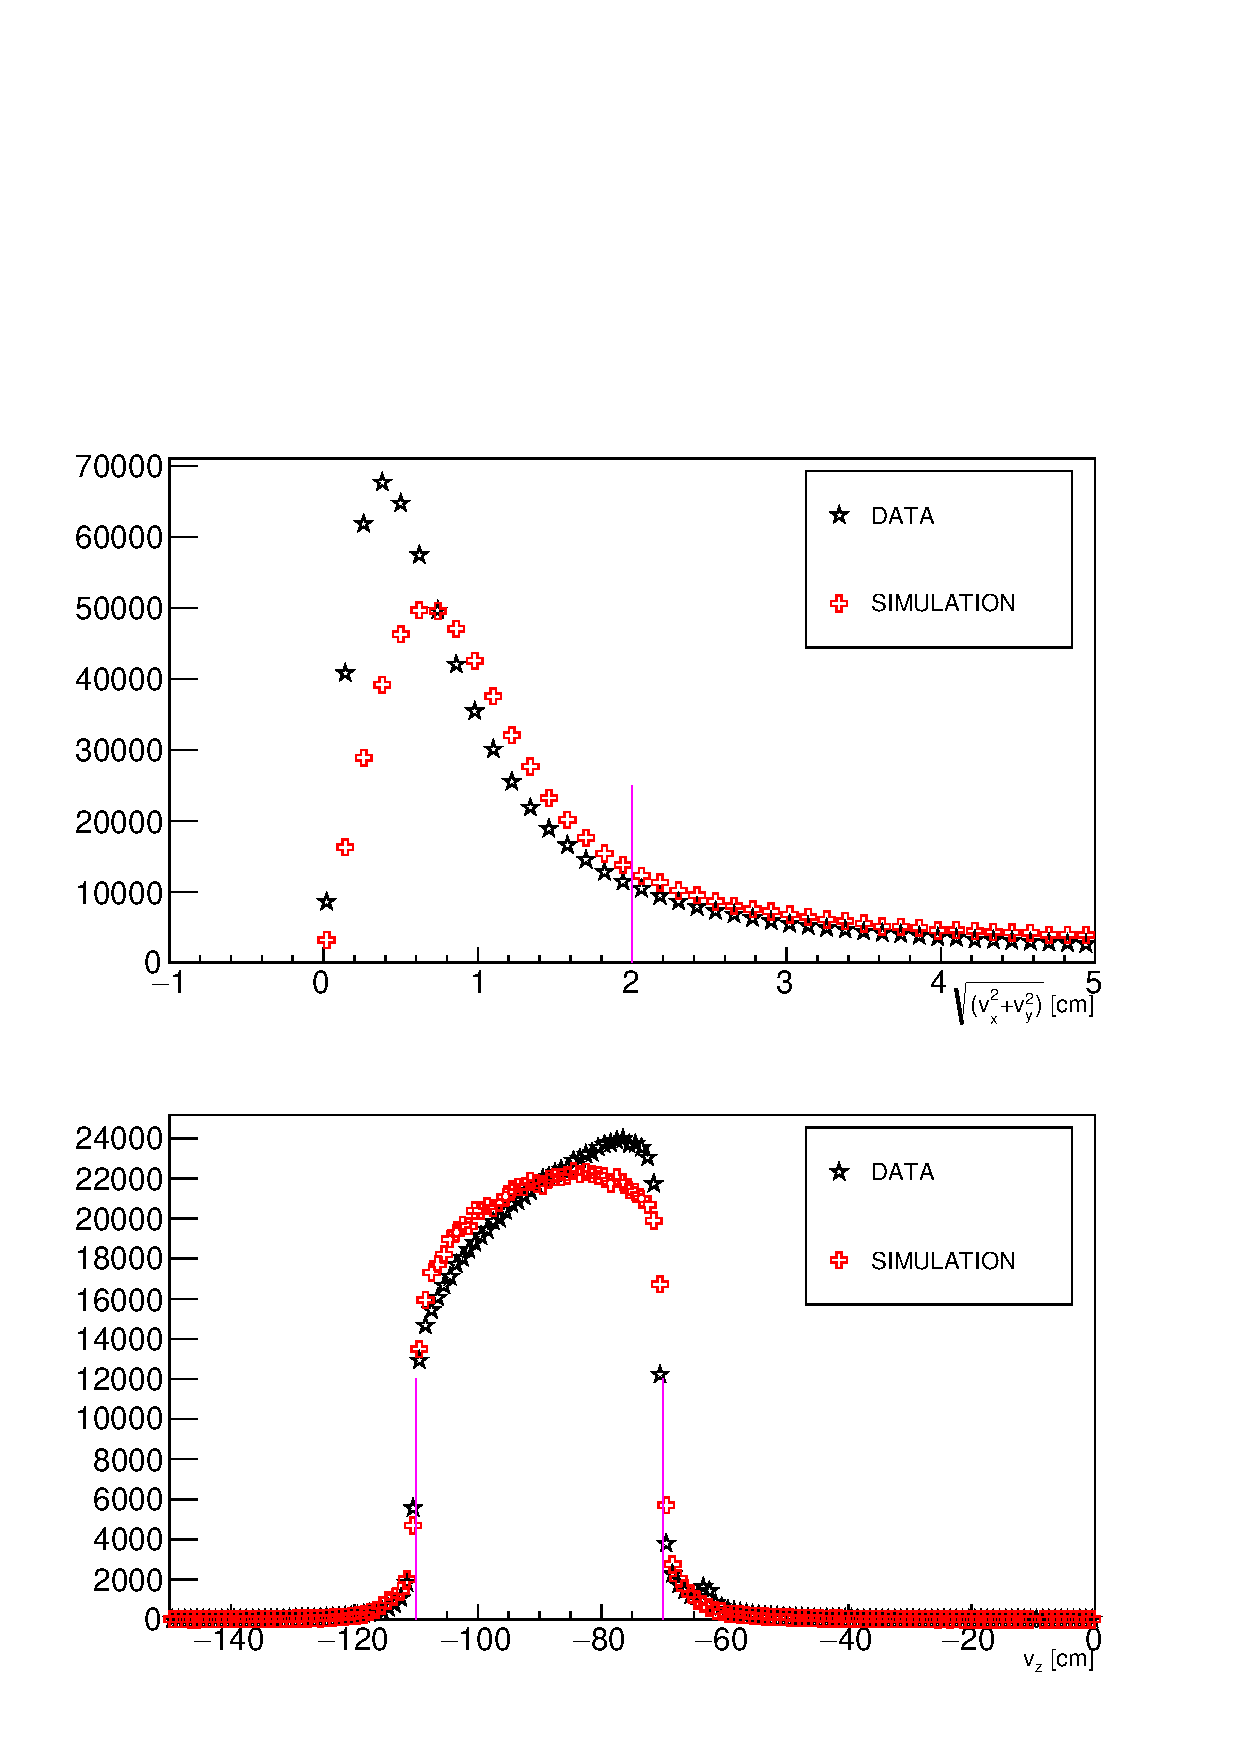
\includegraphics[height=5.8in]{vertex.pdf}}}
\caption{[tpho + tprop -scvt] distribution from the simulation and data for proton, $\pi^{+}$ and $\pi^{-}$.}
\label{Fig1}
\end{figure}

\subsection{Timing Cuts on proton, $\pi^{+}$ and $\pi^{-}$}
\label{TCut}
As a post PID improvement of the detected final state particles $\pi^{+}$, $\pi^{-}$ and proton, we introduced a vertex timing $(t_{vert})$ cut of particles in the analysis. The $t_{vert}$, vertex time is the instant of time the particle left the target. One can calculate it through the information of the TOF detectors as,

\begin{equationarray}
$t_{vert}$(TOF) = t_{TOF}$  -  $\frac{l_{TOF}}{c\beta}$
\end{equationarray}
\\
$\noindent$
where $t_{TOF}$ and ${l_{TOF}$ are the measured time and length of particle in TOF sub detector. Here c is the velocity of light in vacuum and $\beta$ is the Lorentz factor of the particle calculated by knowing the velocity(v) of particle as $\beta = \frac{v}{c}$. The same vertex timing $(t_{vert})$ information can also be calculated from the RF-corrected time instant of the photon ($t_{photon}$)  crossing the target center measure by the tagger added with the t_{prop}$, which is the propagation time from the center of the target to the track vertex. Given by,

\begin{equationarray}
t_{vert}(Tagger) = t_{photon} + t_{prop}.
\end{equationarray}


The difference of the $t_{vert}(TOF)$ from $t_{vert}(Tagger)$ is shown in Fig.$~\ref{Fig2}$, and we make a cut of $\pm$ 1.0 ns around 0 ns for all the final state particles in both simulation and data. 
\begin{figure}[ht!]
\centerline{
\subfloat{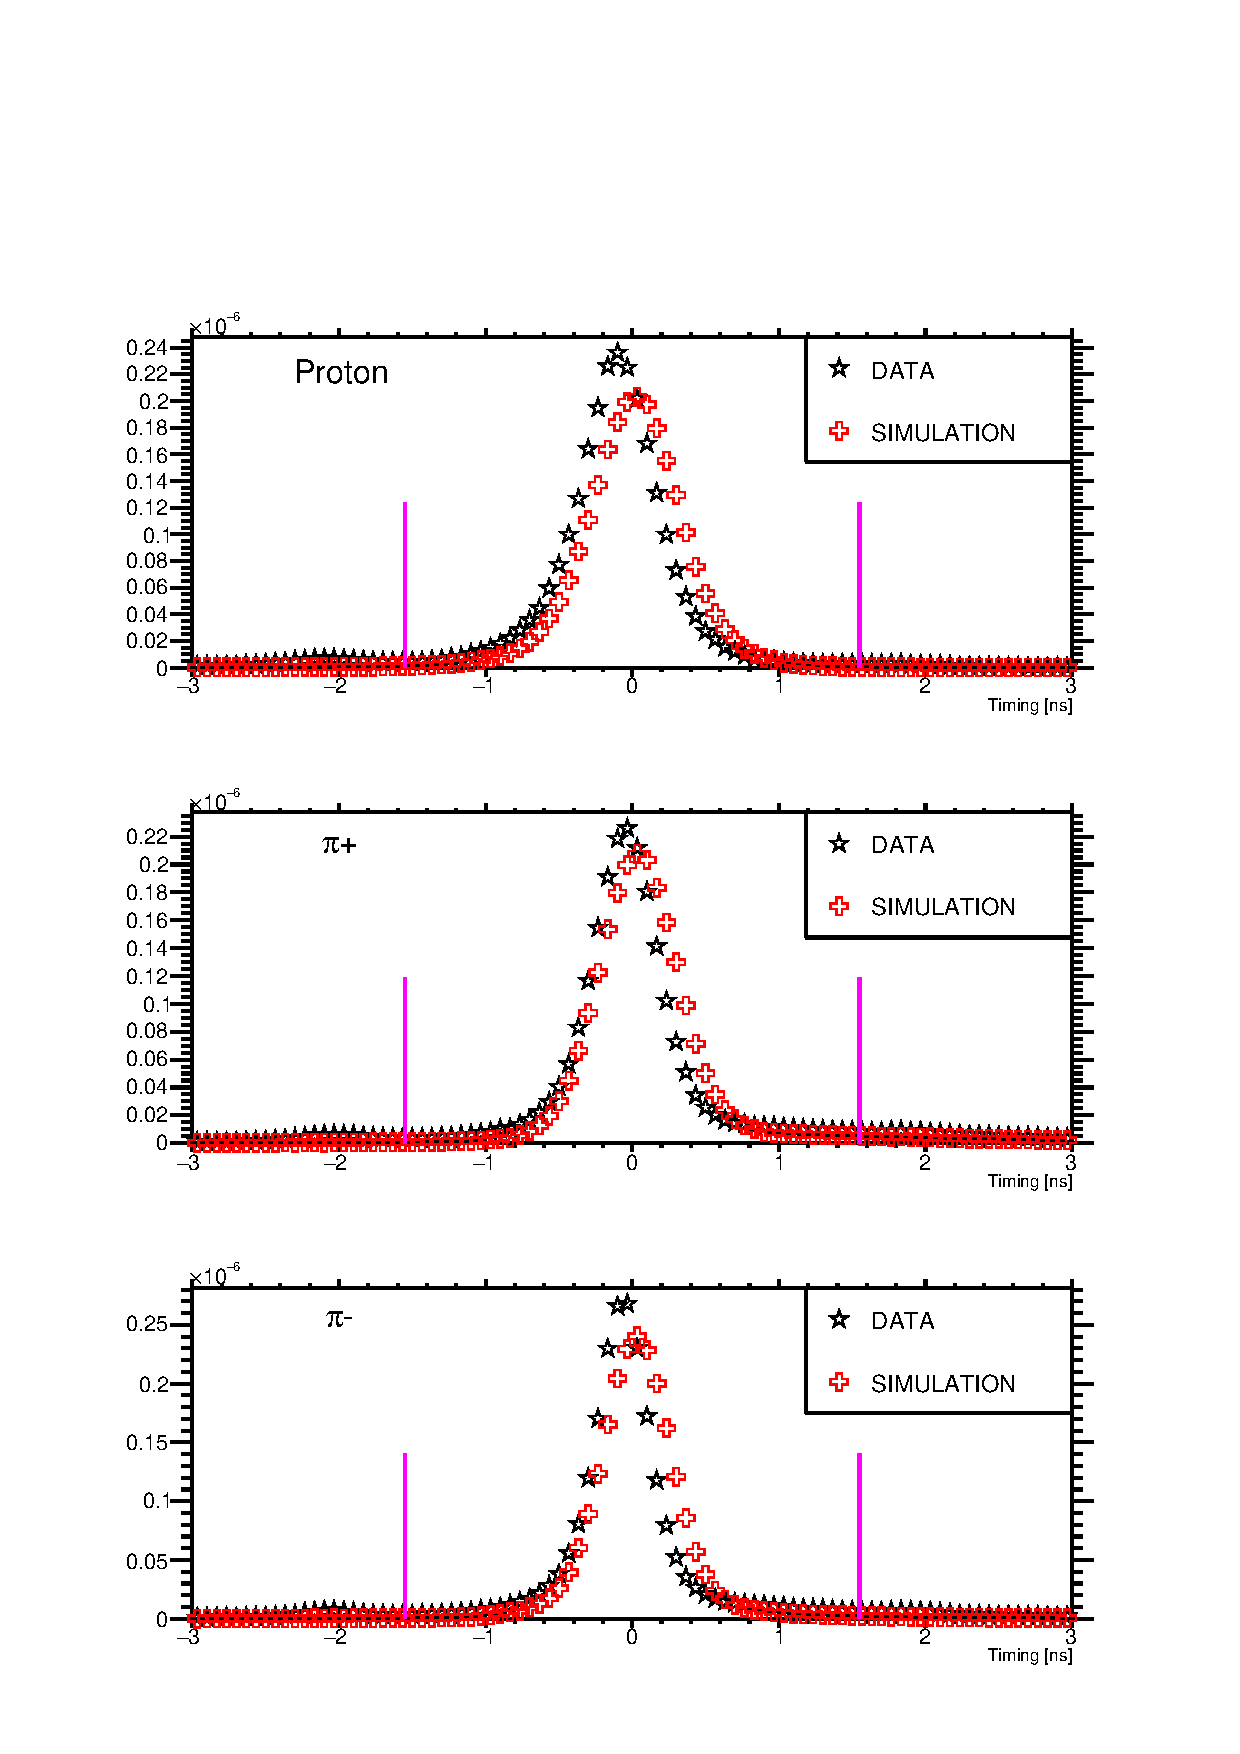
\includegraphics[height=5.8in]{timing.pdf}}}
\caption{[$t_{vert}(TOF)$ - $t_{vert}(Tagger)$] distribution from the simulation and data for proton(Upper), $\pi^{+}$(Middle) and $\pi^{-}$(Lower).}
\label{Fig2}
\end{figure}


\section{G12 Corrections}
\label{Cor}
The G12 Corrections were derived from the exclusive $\pi^{+}$, $\pi^{-}$ and proton reaction. We used the following corrections in the analysis :
    
\begin {itemize}
\item Beam Energy Correction : Is a correction to the incident beam photon energy and dependent on the Run number of the event. This correction is only applicable data and not to the simulated events.
\item Removal of bad TOF paddle : This correction takes the Sector number, Paddle number as input. We used the correction to remove only those paddles that shows a significant drift on the resolutions of particle.   
\item  Geometric Fiducial Cut : This cut removes the dead part of the detector from the $\theta-\phi$ map of the particle. We used it with the "nominal" option. 
\end {itemize}

\subsection{Kinematic Fitting}
\label{KF}
Kinematic fitter is a useful tool often used to get rid of unwanted background from signal channels and helps to improve the signal to background ratio.  Any measurement with a tool comes with an error, and it can be represented as a vector  $\vec{\eta}$. We can also define the measurement as 
\\ $\vec{\eta}$ =  $\vec{y}$. +  $\vec{\epsilon}$.\\
Where the $\vec{y}$ and $\vec{\epsilon}$ denotes the actual value of the measurement without error and $\vec{\epsilon}$ is the error associated with the measurement. The kinematic information of a physics channel along with the constrains imposed allows the fitter to calculate the probability and $\chi^{2}$ of each event using Lagrange multipliers to perform a least-squares fit. The CLAS g12 Kinematic fitter takes the ``TBER (Track Based Error)" matrix, vertex of information and lorentzvector of all particles as input, and returns Pull probabilities and $\chi^{2}$ for each events. The Pull probabilities when fitted with Guassian, its mean and $\sigma$ decides the quality of the covariance matrix and kinematic fit. In the ideal case of gaussian fitted to the Pulls of the particles should have  zero mean and $\sigma$ of one, which ensures that the fitter correctly calculates covariance matrix error. 
  
\begin{figure}[ht!]
\centerline{
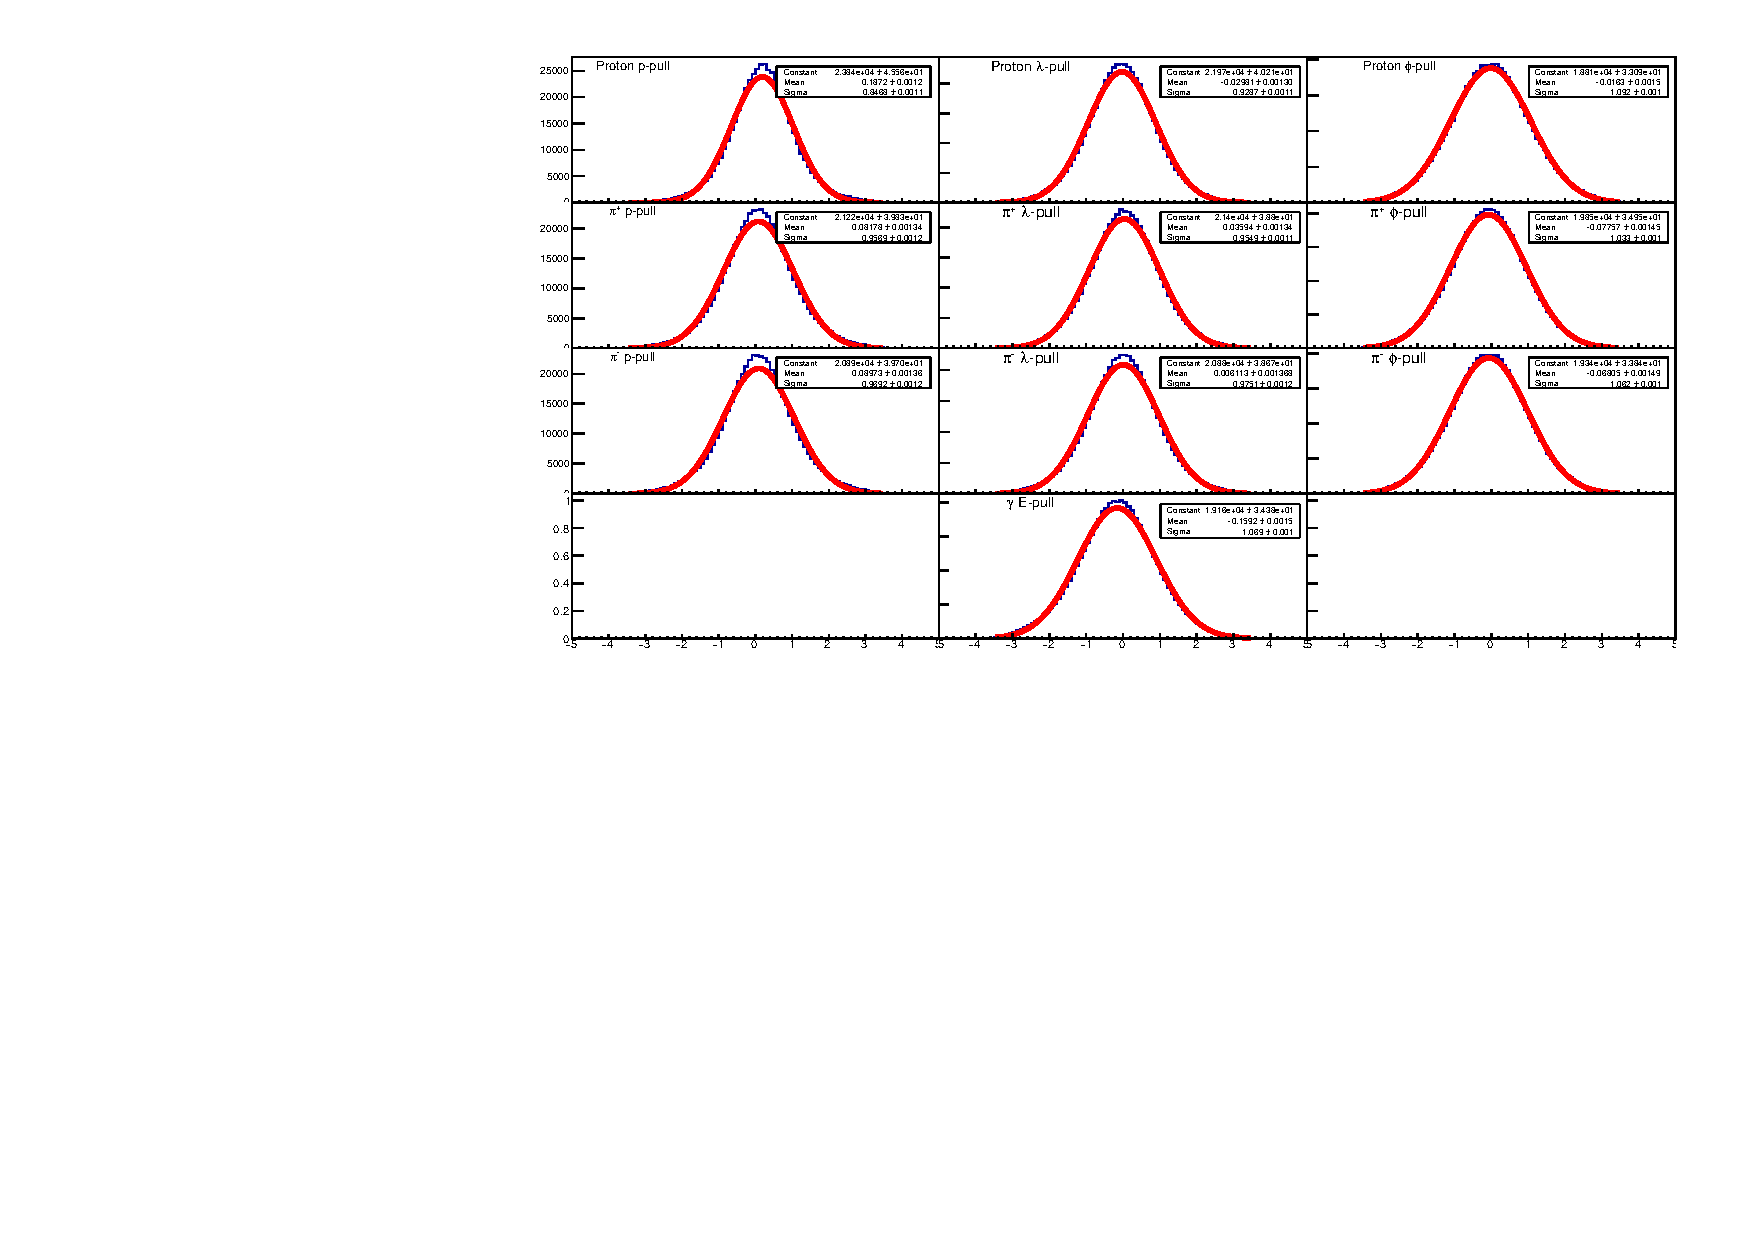
\includegraphics[width=12cm,height=10cm]{Pulls_nothing.pdf}}
\caption{The Pull distributions for a (4-C) kinematic fit to $\gamma$ p $\rightarrow$ $\pi^{+}$ $\pi^{-}$ p from g12 data with run 56655 after a 1$\%$ Pull probability cut.}
\label{Fig3}
\end{figure}

\begin{figure}[ht!]
\centerline{
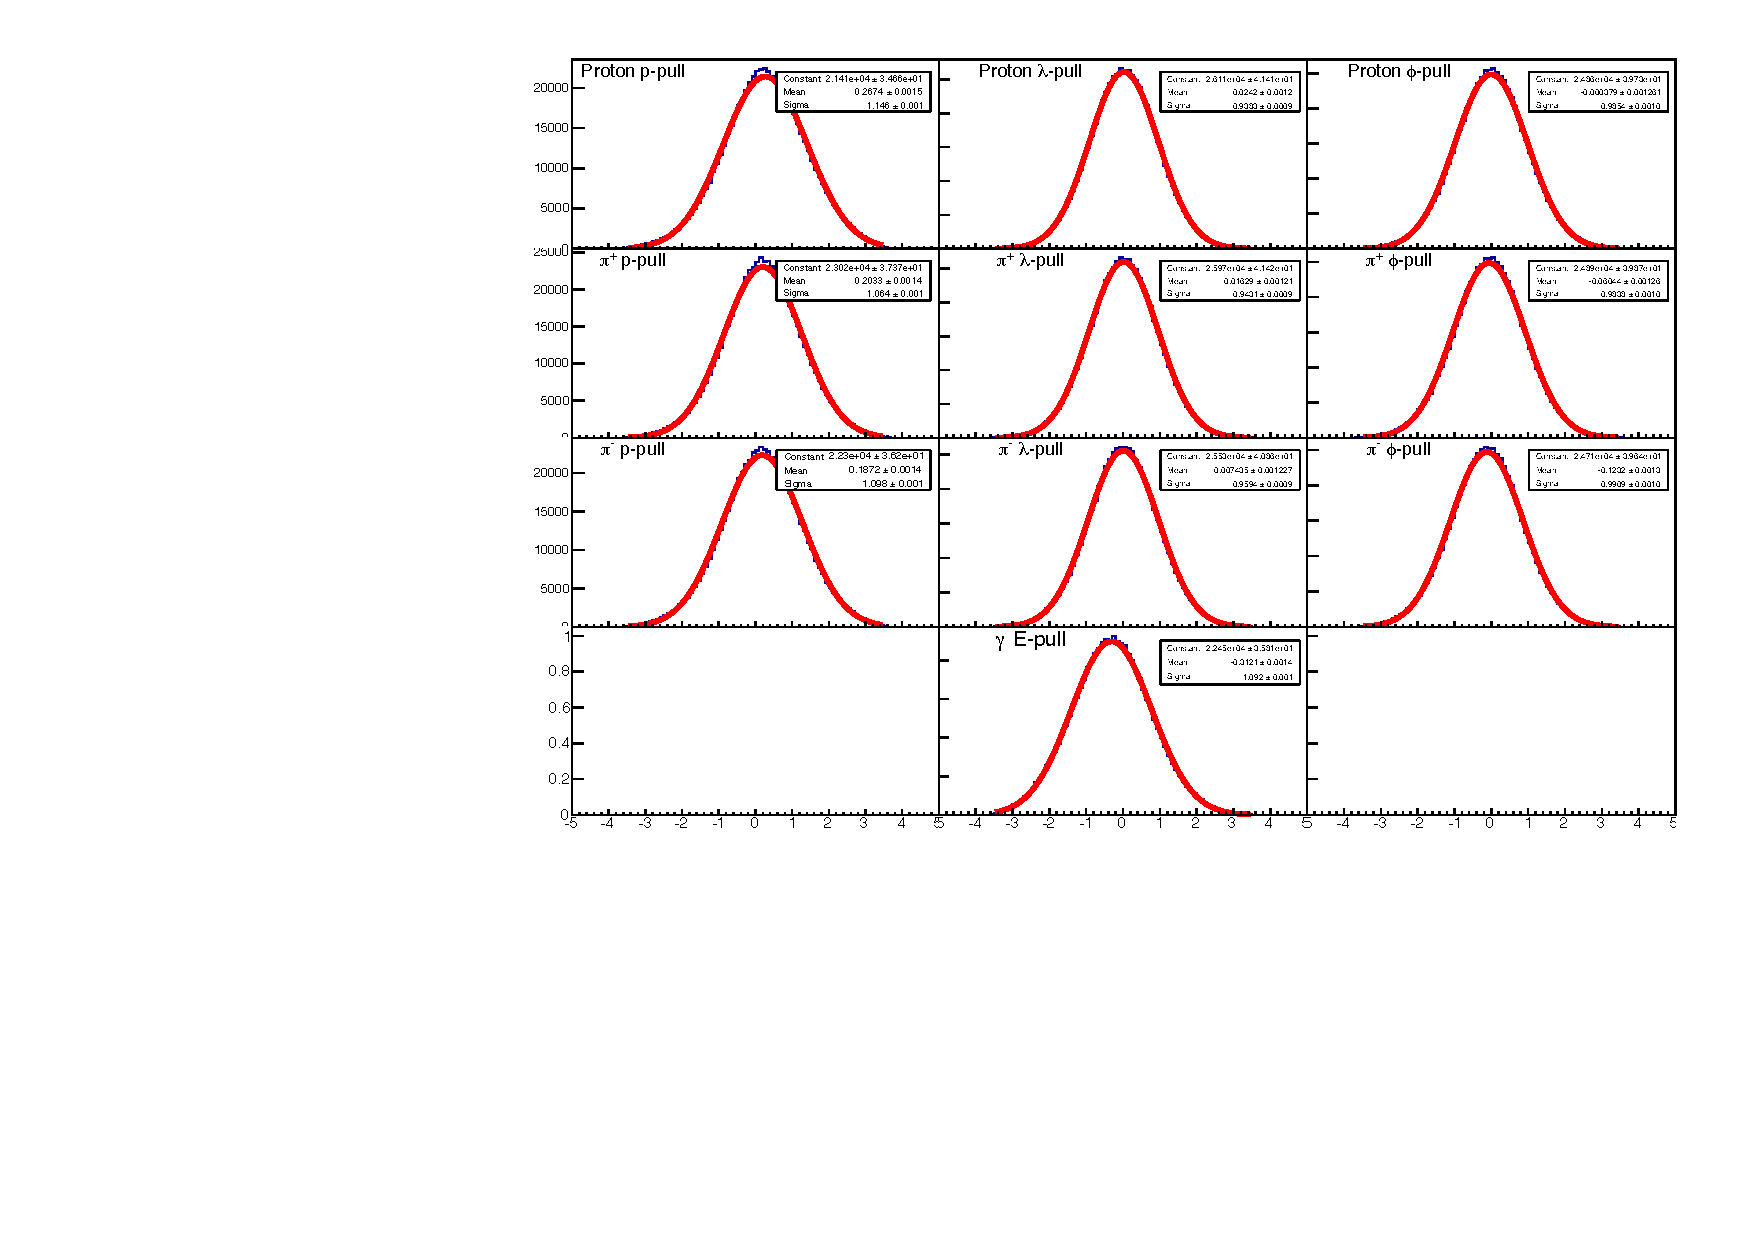
\includegraphics[width=12cm,height=10cm]{SIM_Pulls_nothing.pdf}}
\caption{The Pull distributions for a (4-C) kinematic fit to $\gamma$ p $\rightarrow$ $\pi^{+}$ $\pi^{-}$ p from g12 simulation after a 1$\%$ Pull probability cut.}
\label{Fig4}
\end{figure}
  
The CLAS g12 Kinematic fitter is tuned for 4C constrained reaction,

\begin{equationarray}
$\gamma$ p $\rightarrow$ $\pi^{+}$ $\pi^{-}$ p. 
\end{equationarray}\\
\noindent
The tuning were done for $\pi^{+}$ $\pi^{-}$ and p individually. To check the quality of covariance matrix we have shown the tuned pulls of the particles $\pi^{+}$, $\pi^{-}$ and p from the reaction hypothesis for the data with run 56655 and simulation after a 1$\%$ pull probability cut. The mean and sigma from of the particles are listed in the Table.~\ref{tab2}.

\begin{table}
\centering
\begin{subtable}{.5\textwidth}
\centering
\caption{ }
\begin{tabular}{ |c|c|c| }
\hline
                                        & \mu   & \sigma \\
                               \hline
Proton p-pull                            & 0.187  & 0.846  \\
\hline
Proton $\lambda$-pull                      & -0.029 & 0.928  \\
\hline
Proton $\phi$-pull                         & -0.016 & 1.092  \\
\hline
$\pi^{+}$ p-pull        & 0.081  & 0.957  \\
\hline
$\pi^{+}$ $\lambda$-pull & 0.035  & 0.954  \\
\hline
\pi^{-} $\phi$-pull    & -0.077 & 1.033  \\
\hline
\pi^{-} p-pull        & 0.089  & 0.969  \\
\hline
\pi^{-} $\lambda$-pull & 0.006  & 0.975  \\
\hline
\pi^{-} $\phi$-pull    & -0.068 & 1.062  \\
\hline
$\gamma$ E-pull   & -0.159 & 1.069 \\
\hline
\end{tabular}
\end{subtable}%
\begin{subtable}{.5\textwidth}
\centering
\caption{ }
\begin{tabular}{ |c|c|c| }
\hline
                                         & \mu   & \sigma \\ \hline
Proton p-pull                             & 0.267  & 1.146  \\
\hline
Proton $\lambda$-pull                  & 0.024  & 0.938  \\
\hline
Proton $\phi$-pull                         & -0.000 & 0.985  \\
\hline
$\pi^{+}$ p-pull        & 0.203  & 1.064  \\
\hline
$\pi^{+}$ $\lambda$-pull & 0.016  & 0.943  \\
\hline
$\pi^{+}$ $\phi$-pull    & -0.060 & 0.983  \\
\hline
$\pi^{-}$ p-pull        & 0.187  & 1.098  \\
\hline
$\pi^{-}$ $\lambda$-pull & 0.007  & 0.959  \\
\hline
$\pi^{-}$ $\phi$-pull    & -0.123 & 0.990  \\
\hline
$\gamma$ E-pull                           & -0.312 & 1.092  \\ 
\hline
\end{tabular}
\end{subtable}%
\caption{The table shows the Gaussian mean ($\mu$) and width ($\sigma$) for the pull distributions from a 4C kinematic fit of  $\gamma$ p $\rightarrow$ $\pi^{+}$ $\pi^{-}$ to events from (A) data run 56655 and (B) from simulation after a 1$\%$ Pull probability cut.} 
\label{tab2}
\end{table}

\subsubsection{Fit to the Analysis}

	We use the tuned Kinematic fitter for the 4C constrained fit described above to the reaction hypothesis for our channel 
\begin{equationarray}
$\gamma$ p $\rightarrow$ $(\eta)_{Missing}$ $\pi^{+}$ $\pi^{-}$ p.
\end{equationarray}\\	
 We required the M_{x}(p$\pi^{+}$$\pi^{-}$) has to be an $\eta$ meson. Our reaction hypothesis has the same set of final state particles as for the tuned channel, hence we can comfortably use it without tuning it for our reaction hypothesis again. The Pull probability for the channel of our interest is shown in Fig.~\ref{Fig5} and the dotted line at 0.01 shows the 1$\%$ Pull probability cut to reject events. 
 
\subsection{Simulation}
Pluto, an event generator is used for this analysis. Pluto uses ROOT based programmes very commonly used in Hadron Physics experiments to generate hadronic production and decay. It gives user the freedom to include physics models with simple C++ based codes and to obtain outputs in any desired format. Our simulated events are modelled with bremsstrahlung photon, differential cross-section of $\eta^{\prime}$ and Dalitz plot parameters of $\eta^{\prime}$ \rightarrow$ \eta$ \pi^{+}$ \pi^{-}$ decay. We took the output of the PLUTO program in standared CLAS "gamp" file and processed it with CLAS simulation suit :

\begin {itemize}
\item The gamp files are first converted into the format of PART bank containing the event.
\item GSIM:  Geant3-based simulation in CLAS simulates the decay tracks of particles through the simulation and finally the digitized informations is sorted in the simulated ``raw" banks.
\item GPP: GSIM post-processor smears detector signal more accurately to reflect the actual resolution and to simulate the experimental conditions.  
\item a1c : It is used for reconstruction of simulated data and is the same program used during data reconstruction.
\end {itemize}

The simulated events are then passed through same conditions of Section.~\ref{VCut}, Section.~\ref{TCut}, Section.~\ref{Cor} and Section.~\ref{KF}.
  
\begin{figure}[ht!]
\centerline{
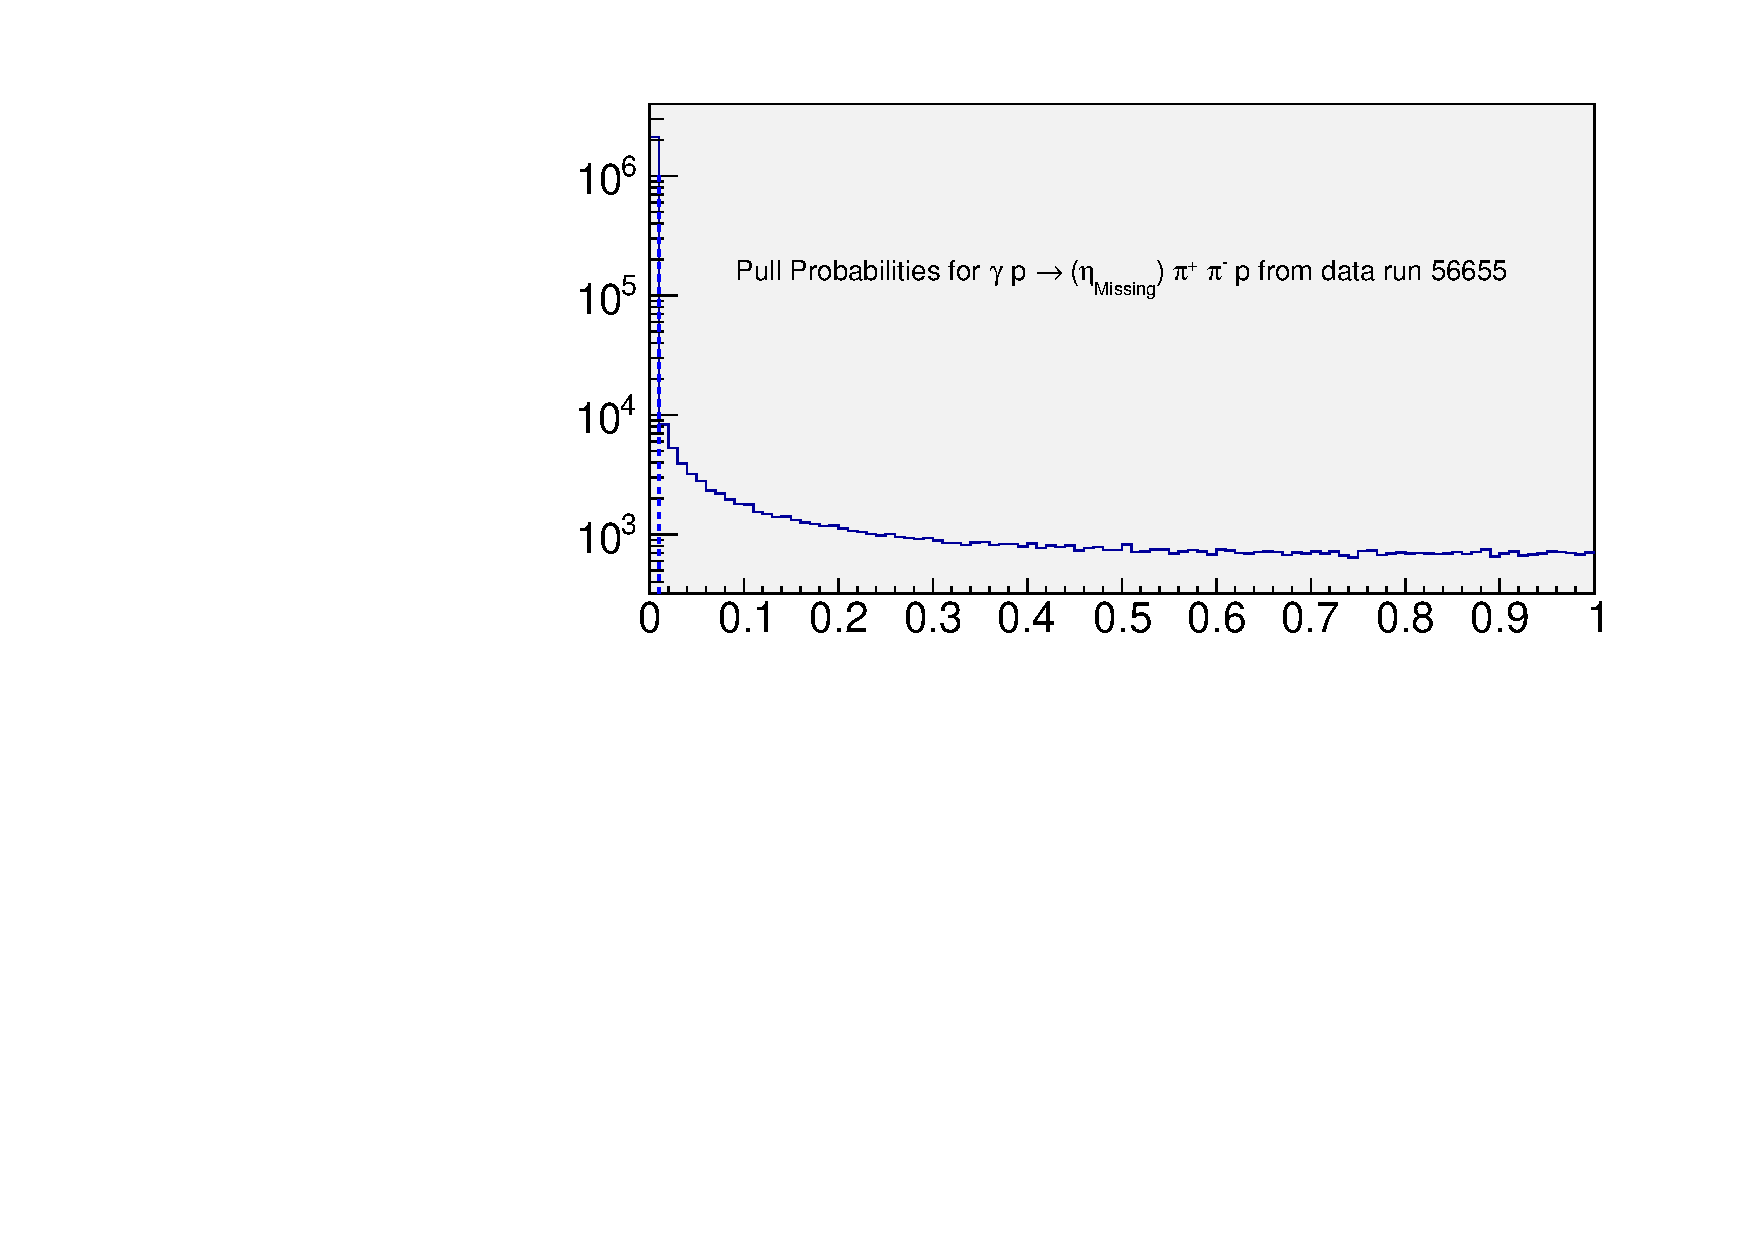
\includegraphics[width=12cm,height=8cm]{Prob_etafit.pdf}}
\caption{The Pull probability for a (1-C) kinematic fit to $\gamma$ p $\rightarrow$ ($\eta_{Missing})$ $\pi^{+}$ $\pi^{-}$ p from data run 56655.}
\label{Fig5}
\end{figure}
 
\begin{table}[]
\centering
\begin{tabular}{|c|c|c|}
\hline
Cuts                                        & g12 Run 56655                    & Simulation \\
\hline
Generated                               & ---                          & 10001500   \\
Reconstructed                           & 42947                        & 855447     \\
Vertex Cut                              & 20092                        & 505405     \\
Timing Cut                              & 11390                        & 451470     \\
Multiple $E_{\gamma}$ & 14986 & ---            \\
Fiducial Cuts                           & 10541                        & 276432     \\
Prob((\eta)\pi^{+}\pi^{-}p) \textgreater 0.01                & 1901                         & 259136    \\
\hline
\end{tabular}
\caption{The table shows the cut flow of the analysis from g12 data run 56655 and simulated events.}
\label{my-label}
\end{table}
 
\end{document}
